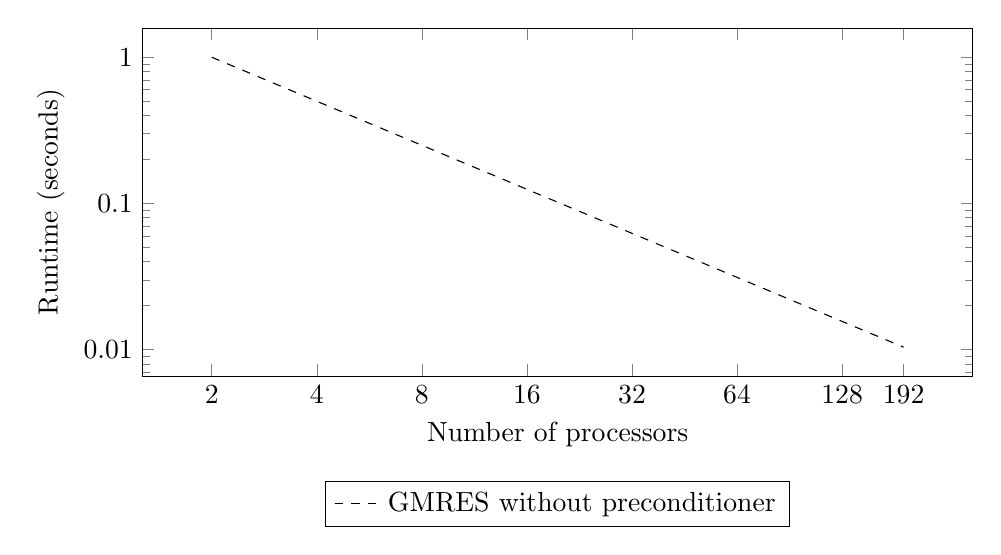
\begin{tikzpicture}
 \begin{axis}[
  height=6cm,
  width=\textwidth,
  xlabel=Number of processors,
  xtick={2, 4, 8, 16, 32, 64, 128, 192},
  xmode=log,
  ymode=log,
  log ticks with fixed point,
  ylabel=Runtime (seconds),
  legend style={
   at={(0.5, -0.3)},
   anchor=north
  }]
   \addplot[color=blue, mark=x] coordinates {
    (2, 0)
    (4, 0)
    (8, 0)
    (16, 0)
    (32, 0)
    (64, 0)
    (96, 0)
    (128, 0)
    (160, 0)
    (192, 0)
   };
   \addlegendentry{GMRES without preconditioner}
   \addplot[color=red, mark=o] coordinates {
    (2, 0)
    (4, 0)
    (8, 0)
    (16, 0)
    (32, 0)
    (64, 0)
    (96, 0)
    (128, 0)
    (160, 0)
    (192, 0)
   };
   \addlegendentry{GMRES + RAS with GMRES on subdomains}
   \addplot[color=yellow, mark=triangle*] coordinates {
    (2, 0)
    (4, 0)
    (8, 0)
    (16, 0)
    (32, 0)
    (64, 0)
    (96, 0)
    (128, 0)
    (160, 0)
    (192, 0)
   };
   \addlegendentry{GMRES + RAS with LU factorisation on subdomains}
   \addplot[color=black, domain=2:192, dashed] expression {
    1*2/x};
   \addlegendentry{Linear speedup}
 \end{axis}
\end{tikzpicture}
